%%%%%%%%%%%%%%%%%%%%%%%%%%%%%%%%%%%%%%%%%%%%%%%%%%%%%%%%%%%%%%%%%%%%%%%%%%%%%%%%%%%%
%Do not alter this block of commands.  If you're proficient at LaTeX, you may include additional packages, create macros, etc. immediately below this block of commands, but make sure to NOT alter the header, margin, and comment settings here. 
\documentclass[12 pt]{article}
\usepackage[margin=1in, top=1.25in, bottom=1.25in]{geometry} 
\usepackage{amsmath,amsthm,amssymb,amsfonts, enumitem, fancyhdr, color, comment, graphicx, environ, bm, tikz}
\usepackage[mathscr]{euscript}
\pagestyle{fancy}
\setlength{\headheight}{25pt}
\newenvironment{problem}[2][Problem]{\begin{trivlist}
\item[\hskip \labelsep {\bfseries #1}\hskip \labelsep {\bfseries #2.}]}{\end{trivlist}}
\newenvironment{sol}
    {\emph{Solution:}
    }
    {
    \qed
    }
\specialcomment{com}{ \color{blue} \textbf{Comment:} }{\color{black}} %for instructor comments while grading

\newtheorem{theorem}{Theorem}
\newtheorem*{corollary}{Corollary}
\newtheorem*{proposition}{Proposition}
\theoremstyle{definition}
\newtheorem*{definition}{Definition}

\NewEnviron{probscore}{\marginpar{ \color{blue} \tiny Problem Score: \BODY \color{black} }}
%%%%%%%%%%%%%%%%%%%%%%%%%%%%%%%%%%%%%%%%%%%%%%%%%%%%%%%%%%%%%%%%%%%%%%%%%%%%%%%%%



\newenvironment{amatrix}[1]{%
  \left[\begin{array}{@{}*{#1}{c}|c@{}}
}{%
  \end{array}\right]
}


%%%%%%%%%%%%%%%%%%%%%%%%%%%%%%%%%%%%%%%%%%%%%
%Fill in the appropriate information below
\fancyhf{}
\lhead{Justin Baum}  %replace with your name
\rhead{Math 544 \\ Spring 2019 \\ Homework 9} %replace XYZ with the homework course number, semester (e.g. ``Spring 2019"), and assignment number.
\lfoot{\thepage}
%%%%%%%%%%%%%%%%%%%%%%%%%%%%%%%%%%%%%%%%%%%%%


% The following are definitions for shortcuts for pieces of notation that I use a lot.
\newcommand{\N}{\mathbb{N}} % the natural numbers
\newcommand{\Z}{\mathbb{Z}} % the integers
\newcommand{\C}{\mathbb{C}} % the complex numbers 
\newcommand{\R}{\mathbb{R}} % the real numbers
\newcommand{\Q}{\mathbb{Q}} % the rational numbers
\newcommand{\F}{\mathbb{F}} % the Field
\renewcommand{\a}{\alpha}
\newcommand{\lin}[1]{\mathscr{L}(#1)}
\newcommand{\lgr}{\lambda}
\newcommand{\vv}[1]{\mathbf{v_{#1}}}
\newcommand{\vu}[1]{\mathbf{u_{#1}}}
\newcommand{\ve}[1]{\mathbf{#1}}
\newcommand{\poly}[2]{\mathscr{P}_#2(#1)}
\newcommand{\zero}{\textbf 0}
\newcommand{\vo}[1]{\mathbf{#1}}
\DeclareMathOperator{\rank}{rank}
\DeclareMathOperator{\range}{range}
\DeclareMathOperator{\nul}{null}
\DeclareMathOperator{\img}{img}


%%%%%%%%%%%%%%%%%%%%%%%%%%%%%%%%%%%%%%
%Do not alter this block.
\begin{document}
%%%%%%%%%%%%%%%%%%%%%%%%%%%%%%%%%%%%%%
\begin{problem}{3.4.10}
Prove that if $T\in\mathscr{L}(V,W)$ and $V$ is finite dimensional, then $T$ is injective iff $\rank T = \dim V$.
\end{problem}
\begin{sol}
If $T$ is injective, then $\ker T = \{\vo{0}\}$, thus by the Rank-Nullity Theorem
\[\dim V = \rank T + \nul T = \rank T\]
If $\dim V = \rank T$, then again by the Rank-Nullity Theorem, 
\[\dim V - \rank T = \nul T = 0\]
Thus $T$ is injective as $\ker T = \{\vo{0}\}$, by definition that the $0$ dimension space is just $\{\vo{0}\}$.
\end{sol}
%%%%%%%%%%%%%%%%%%%%%%%%%%%%%%%%%%%%%%
\begin{problem}{3.4.12}
Suppose that, for a given $A\in \mathscr{M}_3(\R)$, there is a plane $P$ through the origin in $\R^3$ such that the linear system $A\vo{x}=\vo{b}$ is consistent if and only if $\vo{b}\in P$. Prove that the set of solutions of the homogeneous system $A\vo{x}=\vo{0}$ is a line through the origin in $\R^3$.
\end{problem}
\begin{sol}
By the Rank-Nullity Theorem, we know that the $\range A = P$. A plane has dimension $2$. Thus $\dim A - \nul A = \nul A = 1$. The dimension of the nullspace is 1, which means it has a basis of 1 vector, let this vector be $\vv$. The line spanned by $\left <\vv \!\right >=\{a\vv\ |\ a\in \R\}$. This line includes the origin, $a=0$, $\vo{0} \in \left < \vv \!\right >$.
\end{sol}
%%%%%%%%%%%%%%%%%%%%%%%%%%%%%%%%%%%%%%
\begin{problem}{3.4.14}
Suppose that $\dim V = n$ and $S,T\in\lin{V}$.
\begin{enumerate}[label=(\alph*)]
    \item Show that if $\rank ST < n$, then $\rank TS < n$.
    \item Show that if 0 is an eigenvalue of ST, then 0 is an eigenvalue of $TS$.
\end{enumerate}
\end{problem}
\begin{sol}
\begin{enumerate}[label=(\alph*)]
    \item Because $S,T\in \lin{V}$, by proposition 3.30, $\rank S,T \leq \dim V$. Let $\rank TS \geq n$. By proposition 3.30, $\rank S, \rank T \leq \dim V$, thus $\rank S = \rank T = n$. Then by the Rank-Nullity Theorem, $\rank TS = \dim V - \dim(\ker T \cup T^{-1}(\ker S))$. (This is an abuse of notation, $T^{-1}(\ker S) = \{\vo{x}\in V\  |\ T\vo{x}\in \ker S\}$. We already know that $\ker T = \ker S = \{0\}$. Then $\rank ST = \dim V - \nul S - \nul T = \dim V$. Which means the statement $\rank ST \geq n$ is true.
\begin{center}
    \begin{tikzpicture}[scale=1]
        \coordinate (VS)    at (2,0);
        \coordinate (VT)    at (7,0);
        \coordinate (VTS)    at (12,0);
        \draw (VS) circle (2);
        \draw (VS) circle (0.75);
        \draw (VT) circle (0.75);
        \node at (2,0.9) {$\ker T$};
        \node at (7,0.9) {$\ker S$};
        \node at (2,2.40) {V};
        \node at (7,2.40) {V};
        \node at (12,2.40) {V};
        \node at (VS) {$\vo{0}$};
        \node at (VT) {$\vo{0}$};
        \node at (VTS) {$\vo{0}$};
        \draw (VT) circle (2);
        \draw (VT) circle (1.5);
        \node at (2,2.40) {V};
        \node at (7,1.6) {$\img T$};
        \draw (VTS) circle (2);
        \node at (12,1.6) {$\img S$};
        \node at (12,0.7) {$\img TS$};
        \node at (2,2.40) {V};
        \draw[thick,->] (2,0.5) -- (VT);
        \draw[thick,->] (2,1.5) -- (7,1.2);
        \draw (VTS) circle (0.6);
        \draw (VTS) circle (1.5);
        \draw[thick, ->] (7,0.5) -- (VTS);
        \draw[thick, ->] (7, 1.2) -- (12, 0.4);
        %\node[circle,draw=black, fill=white, inner sep=0pt,minimum size=5pt] (b) at () {};
    \end{tikzpicture}
\end{center}
\begin{proposition}{3.30}
If $T\in\lin{V,W}$, then $\rank T \leq \min (\dim V, \dim W)$.
\end{proposition}
    \item Let $\vv{}\neq\vo{0}\in V$ so $ST\vv{}=\vo{0}$. Either $T(\vv{})\in\ker S$ or $T(\vv{})=\vo{0}$. If $T(\vv{})=\vo{0}$ then take $\vo{w}\in V$ so $S(\vo{w})=\vv{}$.  Then $TS \vo{w} = \vo{0}$.\\
    If $T(\vv{})\in \ker S$ then let $\vu{}\in V$, so $S{\vu{}}=\vv{}$. Then $TS\vu{}=\vo{0}$.\\
    If $\nexists \vo{w} : S(\vo{w})=\vv$, then the nullspace of $S$ consists of non-zero vectors, thus it has a eigenvalue of $0$ for all vectors in the nullspace. This is because then $S$ is no longer injective. Thus $\rank S \neq \dim V$ by the Rank-Nullity Theorem, $\nul S \geq 1$.\\
    If $\nexists \vu{} : S(\vu{})=\vv{}$, then by the same argument as for above, there exists an eigenvalue of $0$ for $TS$.\\
    Note: The eigenvectors are not necessarily the same.
\end{enumerate}

\end{sol}
%%%%%%%%%%%%%%%%%%%%%%%%%%%%%%%%%%%%%%
\begin{problem}{3.5.12}
\\ \\  
\begin{enumerate}[label=(\alph*)]
    \item Show that $\mathscr{B}=(1,x,\frac{3}{2}x^2-\frac{1}{2})$ is a basis of $\poly{\R}{2}$.
    \item Find the coordinate representation of $x^2$ with respect to $\mathscr{B}$.
    \item Let $D:\poly{\R}{2}\to\poly{\R}{2}$ be the derivative operator. Find the coordinate representation of D with respect to $\mathscr{B}$.
    \item Use your answers to the last two parts to calculate $\frac{d}{dx}(x^2)$.
\end{enumerate}
\end{problem}
\begin{sol}
\begin{enumerate}[label=(\alph*)]
    \item Let $T: \poly{\R}{2}\to \R^3$ so $T(ax^2+bx+c)=\begin{bmatrix}
    a\\b\\c
    \end{bmatrix}$. Let $A=[T(\mathscr{B_1})|\dots|\mathscr{B_3}]$.
    \[A=\begin{bmatrix}
    0 & 0 & \frac{3}{2}\\
    0 & 1 & 0\\
    1 & 0 & \frac{-1}{2}
    \end{bmatrix}\]
    \newcommand{\vb}[1]{\vo{b_{#1}}}
    In RREF, $A=I_3$. Thus it is a basis.
    \item If $\mathscr{B}=(1,x,\frac{3}{2}x^2-\frac{1}{2})$, let $\vb{1}=1$, $\vb{2}=x$, $\vb{3}=\frac{3}{2}x^2-\frac{1}{2}$.\\
    Then $x^2=\frac{2}{3}(\frac{3}{2}x^2-\frac{1}{2})+\frac{1}{3}(1)=\frac{2}{3}\vb{3}+\frac{1}{3}\vb{1}$. So $x^2 = \begin{bmatrix}
    \frac{1}{3 }\\0\\\frac{2}{3}
    \end{bmatrix}$. If we use $\vb{i}$ as bases for the coordinate representation.
    \item $D:\poly{\R}{2}\to\poly{\R}{2}$, $D(ax^2+bx+c) = 2ax+b$. $\vb{d1}=0$, $\vb{d2}=1$, $\vb{d3}=3x$.
    \item Thus $\begin{bmatrix}
    \frac{1}{3 }\\0\\\frac{2}{3}
    \end{bmatrix}$ with the representation and new bases, is equal to $\frac{1}{3}\vb{d1}+\frac{2}{3}\vb{d3}=2x$.
\end{enumerate}
\end{sol}
\end{document}
